\documentclass[10pt]{beamer}
\usetheme[progressbar=frametitle]{metropolis}
%use Fira
\usepackage{fontspec}
\setsansfont{Fira Sans}
\setmonofont{Fira Mono}
%fix textspacings...
\linespread{1.0} % Standard is 1.0, but Beamer often scales this
\setbeamerfont{block body}{size=\small} % Sometimes smaller font helps the 'density'
\addtobeamertemplate{block begin}{\setlength{\parskip}{0pt}}{}
\addtobeamertemplate{block begin}{}{\vspace{-0.5ex}} % add space after title
\addtobeamertemplate{block alerted begin}{}{\vspace{-0.5ex}} % Reduce space after title
\addtobeamertemplate{block example begin}{}{\vspace{-0.5ex}} % Reduce space after title
\setbeamercolor{block title alerted}{bg=} %remove background of alert blocks
%\addtobeamertemplate{block end}{\vspace{-1ex}}{}  % Reduce space after content

% Custom colors
\definecolor{customblue}{RGB}{79, 70, 229}
\definecolor{customlightblue}{RGB}{224, 231, 255}
\definecolor{customgreen}{RGB}{34, 197, 94}
\definecolor{customorange}{RGB}{249, 115, 22}
\definecolor{customred}{RGB}{239, 68, 68}

\definecolor{myDarkTeal}{RGB}{35, 55, 59}
\definecolor{myOrange}{RGB}{235, 129, 27}
\definecolor{myLightGreen}{RGB}{20,176,61}
\definecolor{myLightGray}{RGB}{250,250,250}

%\setbeamercolor{progress bar}{fg=customblue,bg=customlightblue}
%\setbeamercolor{frametitle}{bg=customblue}
%\setbeamercolor{alerted text}{fg=customblue}

\usepackage{tikz}
\usetikzlibrary{arrows.meta,positioning,shapes}


\usepackage{pgfplots}
\pgfplotsset{compat=1.18}

\title{Day 2: Descriptive Statistics \& Probability}
\subtitle{Building the Foundation for Statistical Inference}
\author{}
\date{}

\begin{document}

% Slide 1: Title
\begin{frame}
\titlepage
\begin{center}
\textit{From data to distributions: the mathematical foundation of statistics}
\end{center}
\end{frame}

% Slide 2: Today's Journey
\begin{frame}{Today's Journey}

\begin{block}{Part I: Descriptive Statistics}
\begin{itemize}
\item Summarizing data: central tendency and spread
\item Visualizing distributions
\item Understanding variability in biological data
\end{itemize}
\end{block}

\begin{block}{Part II: Introduction to Probability}
\begin{itemize}
\item Random variables and probability distributions
\item Key distributions for biology
\item Sampling distributions and the Central Limit Theorem
\end{itemize}
\end{block}

\vspace{0.3cm}

\begin{alertblock}{Why This Matters}
These concepts are the \alert{mathematical foundation} for everything that follows: \\
hypothesis testing, confidence intervals, regression, experimental design
\end{alertblock}
\end{frame}

% PART I: DESCRIPTIVE STATISTICS

% Slide 3: Part I Title
\begin{frame}
\begin{center}
\Huge \textbf{Part I} \\
\vspace{0.5cm}
\LARGE Descriptive Statistics
\vspace{0.5cm}

\large \textit{Summarizing and visualizing data}
\end{center}
\end{frame}

% Slide 4: Why Descriptive Statistics
\begin{frame}{Why Descriptive Statistics?}

\begin{block}{The Challenge}
Raw data is overwhelming—we need ways to \alert{summarize} and \alert{communicate} patterns
\end{block}

\vspace{0.3cm}

\begin{exampleblock}{Example: Mouse Weights}
You measure weights (in grams) of 100 mice: \\
\small 23.4, 25.1, 24.8, 26.2, 23.9, 25.5, 24.1, ... (97 more values)

\vspace{0.3cm}
\textbf{Raw data:} Hard to grasp the pattern

\vspace{0.2cm}
\textbf{Descriptive statistics:} \\
Mean = 25.1g, SD = 1.8g, Range = 20.5-29.3g \\
→ Immediately informative!
\end{exampleblock}

\vspace{0.3cm}

\textbf{Goals of descriptive statistics:}
\begin{itemize}
\item Reduce data to key features
\item Detect patterns and outliers
\item Enable comparison across groups
\item Prepare for formal inference
\end{itemize}
\end{frame}

% Slide 5: Measures of Central Tendency
\begin{frame}{Measures of Central Tendency}
\framesubtitle{Where is the ``middle'' of the data?}

\begin{columns}[T]
\begin{column}{0.32\textwidth}
\begin{block}{Mean ($\bar{x}$)}
\textbf{Average:} Sum divided by n

\vspace{0.2cm}
$$\bar{x} = \frac{\sum x_i}{n}$$

\vspace{0.2cm}
\textbf{Pros:}
\begin{itemize}
\item Uses all data
\item Mathematical properties
\end{itemize}

\textbf{Cons:}
\begin{itemize}
\item Sensitive to outliers
\end{itemize}
\end{block}
\end{column}

\begin{column}{0.32\textwidth}
\begin{block}{Median}
\textbf{Middle value} when sorted

\vspace{0.2cm}
50th percentile

\vspace{0.45cm}

\textbf{Pros:}
\begin{itemize}
\item Robust to outliers
\item Intuitive
\end{itemize}

\textbf{Cons:}
\begin{itemize}
\item Ignores much data
\end{itemize}
\end{block}
\end{column}

\begin{column}{0.32\textwidth}
\begin{block}{Mode}
\textbf{Most frequent} value

\vspace{0.2cm}
Peak of distribution

\vspace{0.45cm}

\textbf{Pros:}
\begin{itemize}
\item Works for categorical data
\end{itemize}

\textbf{Cons:}
\begin{itemize}
\item May not be unique
\item Less useful for continuous data
\end{itemize}
\end{block}
\end{column}
\end{columns}

\vspace{0.3cm}

\begin{center}
\textbf{Which to use?} Depends on data distribution and purpose
\end{center}
\end{frame}

% Slide 6: Example - When Measures Differ
\begin{frame}{Example: When Measures Differ}

\begin{columns}[T]
\begin{column}{0.78\textwidth}
\begin{exampleblock}{Gene Expression Data (arbitrary units)}
Sample A: 10, 12, 11, 13, 12, 11, 12, 10, 13, 11 \\
Sample B: 10, 12, 11, 13, 12, 11, 12, 10, 13, \alert{85}

\vspace{0.3cm}
\textbf{Sample A (normal):}
\begin{itemize}
\item Mean = 11.5, Median = 11.5, Mode = 11, 12
\item All measures agree → symmetric distribution
\end{itemize}

\vspace{0.3cm}
\textbf{Sample B (with outlier):}
\begin{itemize}
\item Mean = \alert{18.9} (pulled up by outlier!)
\item Median = 12 (robust to outlier)
\item Mode = 11, 12
\item Mean $\neq$ Median → skewed distribution
\end{itemize}
\end{exampleblock}
\end{column}

\begin{column}{.3\textwidth}
\includegraphics[width=\textwidth]{imgs/outlier.png}
\end{column}

\end{columns}

\vspace{0.1cm}

\begin{alertblock}{Lesson}
Always check if mean and median differ substantially—\\
suggests outliers or skewed data!
\end{alertblock}
\end{frame}

% Slide 7: Measures of Spread
\begin{frame}{Measures of Spread (Variability)}
\framesubtitle{How dispersed is the data?}

\textbf{Range:} Maximum - Minimum
\begin{itemize}
\item Simple but sensitive to extreme outliers
\item Example: Mouse weights 20.5-29.3g → Range = 8.8g
\end{itemize}

\vspace{0.3cm}

\textbf{Variance ($s^2$):} Average squared deviation from mean
$$s^2 = \frac{\sum (x_i - \bar{x})^2}{n-1}$$

\begin{itemize}
\item Units are squared (harder to interpret)
\item Heavily penalizes outliers (squared deviations)
\end{itemize}

\vspace{0.3cm}

\textbf{Standard Deviation ($s$):} Square root of variance
$$s = \sqrt{s^2}$$

\begin{itemize}
\item Same units as original data (easier to interpret)
\item Most common measure of spread
\item Example: Mouse weights SD = 1.8g
\end{itemize}
\end{frame}

% Slide 8: Why n-1?
\begin{frame}{Why Divide by $n-1$ Instead of $n$?}

\begin{block}{The Issue}
Sample variance estimates population variance—but samples underestimate variability
\end{block}

\vspace{0.3cm}

\textbf{Intuition:}
\begin{itemize}
{\small
	\item Sample mean $\bar{x}$ is calculated from the same data
		\item Data points are naturally closer to $\bar{x}$ than to true population mean $\mu$
		\item Dividing by $n$ would systematically underestimate variance
		\item Dividing by $n-1$ corrects this bias (Bessel's correction)
}
\end{itemize}

\vspace{0.3cm}

\begin{exampleblock}{Example}
\vspace{ 0.5cm }

\begin{columns}[T]

\begin{column}{.5\textwidth}
\begin{itemize}
\item sample from a population
\item calculate variance using both estimators
\item compare
\end{itemize}
\end{column}

\begin{column}{.5\textwidth}
\includegraphics[width=\textwidth]{imgs/variance_estimator.png}
\end{column}
\end{columns}


%Population: 1, 2, 3, 4, 5 (true mean = 3, true SD = 1.58) \\
%Sample: 2, 4 (sample mean = 3)

%\vspace{0.2cm}
%Deviation from sample mean: $|2-3| + |4-3| = 2$ (small!) \\
%Deviation from true mean: $|2-3| + |4-3| = 2$ (same by chance, but usually larger)

%\vspace{0.2cm}
%Divide by $n-1$ to get unbiased estimate of population variance
\end{exampleblock}
\end{frame}

% Slide 9: Quartiles and IQR
\begin{frame}{Quartiles and Interquartile Range}

\begin{block}{Quartiles}
Divide ordered data into four equal parts:
\begin{itemize}
\item Q1 (25th percentile): 25\% of data below
\item Q2 (50th percentile): The median
\item Q3 (75th percentile): 75\% of data below
\end{itemize}
\end{block}

\vspace{0.3cm}

\begin{block}{Interquartile Range (IQR)}
$$\text{IQR} = Q3 - Q1$$

\textbf{Middle 50\% of data}—robust measure of spread
\end{block}

\vspace{0.3cm}

\begin{exampleblock}{Example: Cell Sizes}
Cell diameters (μm): 8, 9, 10, 11, 12, 13, 14, 15, 16, 18, 25

\vspace{0.2cm}
Q1 = 10, Q2 = 13, Q3 = 16, IQR = 6 \\
Note: IQR not affected by outlier (25 μm)
\end{exampleblock}
\end{frame}

% Slide 10: Outlier Detection
\begin{frame}{Using IQR to Detect Outliers}

\begin{block}{Common Rule}
Values are potential outliers if:
$$x < Q1 - 1.5 \times \text{IQR} \quad \text{or} \quad x > Q3 + 1.5 \times \text{IQR}$$
\end{block}

\vspace{0.3cm}

\begin{exampleblock}{Example: Cell Sizes (continued)}
Q1 = 10, Q3 = 16, IQR = 6

\vspace{0.2cm}
Lower fence: $10 - 1.5 \times 6 = 1$ \\
Upper fence: $16 + 1.5 \times 6 = 25$

\vspace{0.2cm}
The 25 μm cell is right at the boundary—might be an outlier!
\end{exampleblock}

\vspace{0.3cm}

\begin{alertblock}{Important}
\alert{Don't automatically remove outliers!} They might be:
\begin{itemize}
\item Measurement errors (remove)
\item Real biological variation (keep!)
\item The most interesting observations (investigate!)
\end{itemize}
\end{alertblock}
\end{frame}

% Slide 11: Visualization - Histograms
\begin{frame}{Visualizing Distributions: Histograms}

\begin{columns}[T]
\begin{column}{0.48\textwidth}
\begin{block}{Histogram}
Divides data range into bins, counts observations per bin

\vspace{0.2cm}
\textbf{Shows:}
\begin{itemize}
\item Shape of distribution
\item Central tendency
\item Spread
\item Outliers
\item Skewness
\item Modality (peaks)
\end{itemize}
\end{block}

\begin{alertblock}{Tip}
Try different bin widths—\\
too few bins hide detail, \\
too many show noise
\end{alertblock}
\end{column}

\begin{column}{0.48\textwidth}
\begin{center}
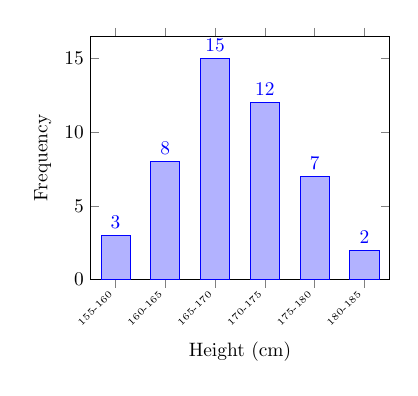
\begin{tikzpicture}[scale=0.7]
\begin{axis}[
    ybar,
    bar width=15pt,
    ylabel={Frequency},
    xlabel={Height (cm)},
    ymin=0,
    symbolic x coords={155-160, 160-165, 165-170, 170-175, 175-180, 180-185},
    xtick=data,
    nodes near coords,
    x tick label style={rotate=45, anchor=east, font=\tiny},
    width=7cm,
    height=6cm
]
\addplot coordinates {
    (155-160, 3)
    (160-165, 8)
    (165-170, 15)
    (170-175, 12)
    (175-180, 7)
    (180-185, 2)
};
\end{axis}
\end{tikzpicture}

\vspace{0.2cm}
\small \textit{Example: Student heights}
\end{center}
\end{column}
\end{columns}
\end{frame}

% Slide 12: Box Plots
\begin{frame}{Box Plots (Box-and-Whisker Plots)}

\begin{columns}[T]
\begin{column}{0.48\textwidth}
\begin{block}{Components}
\begin{itemize}
\item \textbf{Box:} IQR (Q1 to Q3)
\item \textbf{Line in box:} Median
\item \textbf{Whiskers:} Extend to most extreme non-outlier
\item \textbf{Points beyond:} Outliers
\end{itemize}
\end{block}

\vspace{0.3cm}

\textbf{Advantages:}
\begin{itemize}
\item Compact summary
\item Easy group comparisons
\item Shows outliers
\item Distribution-free (no assumptions)
\end{itemize}

\vspace{0.2cm}

\end{column}
\begin{column}{.48\textwidth}
\includegraphics[width=\textwidth]{imgs/variance_estimator_boxplot.png}\\
\end{column}

\end{columns}
\begin{center}
\textbf{Better than bar plots!}
\end{center}
\end{frame}

% Slide 13: Distribution Shapes
\begin{frame}{Understanding Distribution Shapes}

\begin{columns}[T]
\begin{column}{0.32\textwidth}
\begin{block}{Symmetric}
\begin{center}
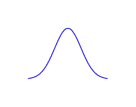
\begin{tikzpicture}[scale=0.5]
\begin{axis}[
    width=4cm, height=3cm,
    axis lines=none,
    ymin=0
]
\addplot[thick, customblue, smooth, domain=-3:3, samples=50] {exp(-x^2/2)};
\end{axis}
\end{tikzpicture}
\end{center}

Mean $\approx$ Median \\
\small Bell-shaped \\
\small \textit{Example: Heights}
\end{block}
\end{column}

\begin{column}{0.32\textwidth}
\begin{block}{Right-Skewed}
\begin{center}
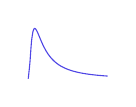
\begin{tikzpicture}[scale=0.5]
\begin{axis}[
    width=4cm, height=3cm,
    axis lines=none,
    ymin=0
]
\addplot[thick, customblue, smooth, domain=0.1:5, samples=50] {(1/x^2)*exp(-1/x)};
\end{axis}
\end{tikzpicture}
\end{center}

Mean $>$ Median \\
\small Long right tail \\
\small \textit{Example: Income}
\end{block}
\end{column}

\begin{column}{0.32\textwidth}
\begin{block}{Bimodal}
\begin{center}
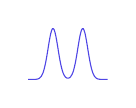
\begin{tikzpicture}[scale=0.5]
\begin{axis}[
    width=4cm, height=3cm,
    axis lines=none,
    ymin=0
]
\addplot[thick, customblue, smooth, domain=-4:4, samples=50] {0.5*exp(-(x+1.5)^2/0.5) + 0.5*exp(-(x-1.5)^2/0.5)};
\end{axis}
\end{tikzpicture}
\end{center}

Two peaks \\
\small Often indicates subgroups \\
\small \textit{Example: Mixed sexes}
\end{block}
\end{column}
\end{columns}

\vspace{0.5cm}

\begin{alertblock}{Why This Matters}
Distribution shape affects:
\begin{itemize}
\item Which summary statistics to use (mean vs. median)
\item Which statistical tests are appropriate
\item How to interpret results
\end{itemize}
\end{alertblock}
\end{frame}

% Slide 14: Skewness in Biology
\begin{frame}{Skewness in Biological Data}

\textbf{Many biological measurements are right-skewed:}

\vspace{0.3cm}

\begin{itemize}
\item \textbf{Gene expression:} Most genes expressed at low levels, few highly expressed
\item \textbf{Cell size:} Bounded at zero, occasional very large cells
\item \textbf{Reaction times:} Bounded at zero, occasional very slow responses
\item \textbf{Survival times:} Most die at similar time, some live much longer
\item \textbf{Pathogen load:} Most hosts have low burden, some very high
\end{itemize}

\vspace{0.4cm}

\begin{exampleblock}{Consequences}
\begin{itemize}
\item Mean pulled toward tail (may not represent typical value)
\item Standard deviation inflated by outliers
\item Violates normality assumption of many tests
\end{itemize}
\end{exampleblock}

\vspace{0.3cm}

\begin{alertblock}{Solution}
Log transformation often helps: $\log(x)$ more symmetric if $x$ is right-skewed
\end{alertblock}
\end{frame}

% Slide 15: Log Transformation
\begin{frame}{Log Transformation}

\begin{block}{When to Use}
Data spans multiple orders of magnitude and/or is right-skewed
\end{block}

\vspace{0.3cm}

\begin{exampleblock}{Example: Bacterial Counts}
\textbf{Raw data:} 100, 500, 1000, 5000, 50000, 500000 CFU/mL \\
\small Highly skewed, hard to visualize

\vspace{0.3cm}
\textbf{Log10 transformed:} 2, 2.7, 3, 3.7, 4.7, 5.7 \\
\small More symmetric, easier to work with

\vspace{0.3cm}
\textbf{Biological interpretation:} \\
Equal steps on log scale = equal fold-changes \\
(e.g., 2 to 3 is 10-fold increase, like 3 to 4)
\end{exampleblock}

\vspace{0.3cm}

\begin{alertblock}{Important}
After analysis on log scale, transform back for reporting: \\
Mean of logs → \alert{geometric mean}, not arithmetic mean
\end{alertblock}
\end{frame}

% Slide 16: Standardization (Z-scores)
\begin{frame}{Standardization: Z-scores}

\begin{block}{Z-score}
Number of standard deviations from the mean:
$$z = \frac{x - \bar{x}}{s}$$
\end{block}

\vspace{0.3cm}

\textbf{Properties:}
\begin{itemize}
\item Mean = 0, SD = 1
\item Dimensionless (removes units)
\item Allows comparison across different scales
\end{itemize}

\vspace{0.3cm}

\begin{exampleblock}{Example: Comparing Variables}
Mouse weight: 25g (mean=24g, SD=2g) → $z = 0.5$ \\
Mouse length: 9cm (mean=10cm, SD=1cm) → $z = -1.0$

\vspace{0.2cm}
Length is more unusual (further from mean in SD units)
\end{exampleblock}

\vspace{0.3cm}

\textbf{Interpretation:}
\begin{itemize}
\item $|z| < 2$: Within typical range
\item $|z| > 2$: Unusual
\item $|z| > 3$: Very unusual (potential outlier)
\end{itemize}
\end{frame}

% Slide 17: Covariance and Correlation
\begin{frame}{Relationships Between Variables}
\framesubtitle{Covariance and Correlation}

\begin{block}{Covariance}
Measure of how two variables vary together:
$$\text{cov}(x,y) = \frac{\sum (x_i - \bar{x})(y_i - \bar{y})}{n-1}$$

\textbf{Problem:} Units depend on scale of variables (hard to interpret)
\end{block}

\vspace{0.3cm}

\begin{block}{Correlation (Pearson's $r$)}
Standardized covariance:
$$r = \frac{\text{cov}(x,y)}{s_x \cdot s_y}$$

\textbf{Properties:}
\begin{itemize}
\item Range: $-1$ to $+1$
\item $r = +1$: Perfect positive linear relationship
\item $r = -1$: Perfect negative linear relationship
\item $r = 0$: No linear relationship
\end{itemize}
\end{block}
\end{frame}

% Slide 18: Interpreting Correlation
\begin{frame}{Interpreting Correlation}

\begin{columns}[T]
\begin{column}{0.48\textwidth}
\textbf{Rules of thumb:}
\begin{itemize}
\item $|r| < 0.3$: Weak
\item $0.3 < |r| < 0.7$: Moderate
\item $|r| > 0.7$: Strong
\end{itemize}

\vspace{0.3cm}

\begin{alertblock}{Critical Reminders}
\begin{itemize}
\item Correlation $\neq$ causation!
\item Only measures \alert{linear} relationships
\item Sensitive to outliers
\item Sample size matters
\end{itemize}
\end{alertblock}
\end{column}

\begin{column}{0.48\textwidth}
\begin{exampleblock}{Biology Example}
\textbf{Body mass vs. metabolic rate:}

\vspace{0.2cm}
$r = 0.92$ (strong positive)

\vspace{0.2cm}
Larger animals have higher metabolic rates

\vspace{0.2cm}
\alert{But:} Correlation doesn't tell us about the \emph{functional form} (actually follows power law, not linear)
\end{exampleblock}

\vspace{0.2cm}

\begin{center}
\textbf{Always plot the data!} \\
\small (Remember Anscombe's Quartet)
\end{center}
\end{column}
\end{columns}
\end{frame}

% Slide 19: Summary - Descriptive Stats
\begin{frame}{Summary: Descriptive Statistics}

\textbf{Key concepts covered:}

\vspace{0.3cm}

\begin{enumerate}
\item \textbf{Central tendency:} Mean, median, mode \\
\small Choose based on distribution shape

\vspace{0.2cm}
\item \textbf{Spread:} Range, variance, SD, IQR \\
\small Quantify variability in data

\vspace{0.2cm}
\item \textbf{Visualization:} Histograms, box plots \\
\small Always look at your data!

\vspace{0.2cm}
\item \textbf{Distribution shapes:} Symmetric, skewed, bimodal \\
\small Affects choice of methods

\vspace{0.2cm}
\item \textbf{Transformations:} Log, standardization \\
\small Make data more analyzable

\vspace{0.2cm}
\item \textbf{Relationships:} Covariance, correlation \\
\small Quantify associations between variables
\end{enumerate}

\vspace{0.3cm}

\begin{center}
\alert{Next: Moving from describing samples to understanding populations}
\end{center}
\end{frame}


% PART II: PROBABILITY

% Slide 1: Part II Title
\begin{frame}
\begin{center}
\Huge \textbf{Part II} \\
\vspace{0.5cm}
\LARGE Introduction to Probability
\vspace{0.5cm}

\large \textit{From randomness to inference}
\end{center}
\end{frame}

% Slide 2: Why Probability?
\begin{frame}{Why Do We Need Probability?}

\begin{alertblock}{The Core Challenge}
Biological data is inherently \alert{variable} and \alert{uncertain}
\end{alertblock}

\vspace{0.3cm}

\textbf{Sources of variability:}
\begin{itemize}
\item \textbf{Biological variation:} No two organisms are identical
\item \textbf{Measurement error:} Instruments aren't perfect
\item \textbf{Sampling:} We observe a subset, not the whole population
\item \textbf{Stochastic processes:} Many biological processes are inherently random
\end{itemize}

\vspace{0.3cm}

\begin{block}{What Probability Provides}
A mathematical framework to:
\begin{itemize}
\item Quantify uncertainty
\item Make predictions despite randomness
\item Distinguish signal from noise
\item Draw inferences from samples to populations
\end{itemize}
\end{block}

\vspace{0.2cm}

\begin{center}
\textbf{Probability is the language of uncertainty in science}
\end{center}
\end{frame}

% Slide 3: Basic Probability Concepts
\begin{frame}{Basic Probability Concepts}

\begin{block}{Probability}
A number between 0 and 1 representing the likelihood of an event:
\begin{itemize}
\item $P = 0$: Impossible
\item $P = 1$: Certain
\item $0 < P < 1$: Uncertain
\end{itemize}
\end{block}

\vspace{0.3cm}

\textbf{Fundamental rules:}

\begin{enumerate}
\item \textbf{Complement rule:} $P(\text{not } A) = 1 - P(A)$

\vspace{0.2cm}
\item \textbf{Addition rule (mutually exclusive):} \\
$P(A \text{ or } B) = P(A) + P(B)$

\vspace{0.2cm}
\item \textbf{Multiplication rule (independent):} \\
$P(A \text{ and } B) = P(A) \times P(B)$
\end{enumerate}

\vspace{0.3cm}

\begin{exampleblock}{Example: Coin Flips}
$P(\text{heads}) = 0.5$, $P(\text{tails}) = 0.5$ \\
$P(\text{2 heads in a row}) = 0.5 \times 0.5 = 0.25$
\end{exampleblock}
\end{frame}

% Slide 4: Random Variables
\begin{frame}{Random Variables}

\begin{block}{Random Variable}
A variable whose value is determined by a random process
\end{block}

\vspace{0.3cm}

\textbf{Two types:}

\begin{columns}[T]
\begin{column}{0.48\textwidth}
\begin{block}{Discrete}
Takes specific values (countable)

\vspace{0.2cm}
\textbf{Examples:}
\begin{itemize}
\item Number of mutations
\item Number of offspring
\item Number of cells
\item Genotype (AA, Aa, aa)
\end{itemize}
\end{block}
\end{column}

\begin{column}{0.48\textwidth}
\begin{block}{Continuous}
Takes any value in a range

\vspace{0.2cm}
\textbf{Examples:}
\begin{itemize}
\item Height
\item Weight
\item Reaction time
\item Gene expression level
\end{itemize}
\end{block}
\end{column}
\end{columns}

\vspace{0.4cm}

\begin{alertblock}{Key Difference}
\textbf{Discrete:} Probability of exact values (e.g., $P(X = 3)$) \\
\textbf{Continuous:} Probability of ranges (e.g., $P(165 < X < 170)$)
\end{alertblock}
\end{frame}

% Slide 5: Probability Distributions
\begin{frame}{Probability Distributions}

\begin{block}{Probability Distribution}
Describes how probabilities are distributed across possible values of a random variable
\end{block}

\vspace{0.3cm}

\textbf{For discrete variables:}
\begin{itemize}
\item \textbf{Probability Mass Function (PMF):} $P(X = x)$
\item Sum of all probabilities = 1
\end{itemize}

\vspace{0.3cm}

\textbf{For continuous variables:}
\begin{itemize}
\item \textbf{Probability Density Function (PDF):} $f(x)$
\item $P(X = x) = 0$ for any specific value!
\item $P(a < X < b) = \int_a^b f(x) dx$ (area under curve)
\item Total area under PDF = 1
\end{itemize}

\vspace{0.3cm}

\begin{center}
\textbf{A distribution completely characterizes the random variable}
\end{center}
\end{frame}

% Slide 6: Expected Value and Variance
\begin{frame}{Expected Value and Variance}

\begin{block}{Expected Value (Mean)}
Long-run average if we repeated the random process infinitely:

\textbf{Discrete:} $E[X] = \mu = \sum x \cdot P(X = x)$ \\
\textbf{Continuous:} $E[X] = \mu = \int x \cdot f(x) dx$
\end{block}

\vspace{0.3cm}

\begin{block}{Variance}
Expected squared deviation from the mean:

$$\text{Var}(X) = \sigma^2 = E[(X - \mu)^2]$$

\textbf{Standard deviation:} $\sigma = \sqrt{\sigma^2}$
\end{block}

\vspace{0.3cm}

\begin{alertblock}{Population vs. Sample}
\begin{itemize}
\item Population parameters: $\mu$, $\sigma^2$ (unknown, fixed)
\item Sample statistics: $\bar{x}$, $s^2$ (observed, vary between samples)
\item Sample statistics \alert{estimate} population parameters
\end{itemize}
\end{alertblock}
\end{frame}

% Slide 7: The Binomial Distribution
\begin{frame}{The Binomial Distribution}
\framesubtitle{Counting successes in fixed trials}

\begin{block}{When to Use}
\begin{itemize}
\item Fixed number of independent trials ($n$)
\item Each trial has two outcomes (success/failure)
\item Probability of success ($p$) is constant
\item Count number of successes ($X$)
\end{itemize}
\end{block}

\vspace{0.3cm}

\textbf{Notation:} $X \sim \text{Binomial}(n, p)$

\textbf{PMF:} $P(X = k) = \binom{n}{k} p^k (1-p)^{n-k}$

\textbf{Mean:} $E[X] = np$

\textbf{Variance:} $\text{Var}(X) = np(1-p)$

\vspace{0.3cm}

\begin{exampleblock}{Biology Example}
Genotyping 10 plants, each has 0.25 probability of being homozygous recessive \\
$X \sim \text{Binomial}(10, 0.25)$ \\
$E[X] = 10 \times 0.25 = 2.5$ plants expected
\end{exampleblock}
\end{frame}

% Slide 8: Binomial Example
\begin{frame}{Binomial Distribution: Detailed Example}

\begin{exampleblock}{Mutation Detection}
\textbf{Scenario:} Sequence 20 DNA samples, each has 0.1 probability of carrying a specific mutation

\vspace{0.3cm}
$X \sim \text{Binomial}(20, 0.1)$ where $X$ = number with mutation

\vspace{0.3cm}
\textbf{Questions we can answer:}

\begin{itemize}
\item What's the most likely outcome? \\
$E[X] = 20 \times 0.1 = 2$ mutations expected

\vspace{0.2cm}
\item What's $P(X = 0)$ (no mutations)? \\
$P(X = 0) = \binom{20}{0} (0.1)^0 (0.9)^{20} = 0.122$ (12.2\%)

\vspace{0.2cm}
\item What's $P(X \geq 5)$ (at least 5 mutations)? \\
$P(X \geq 5) = 1 - P(X < 5) = 0.043$ (4.3\%)
\end{itemize}
\end{exampleblock}

\vspace{0.2cm}

\textbf{Interpretation:} If we see 5+ mutations, it's unusual (only 4.3\% chance), suggesting $p$ might be higher than 0.1!
\end{frame}

% Slide 9: The Poisson Distribution
\begin{frame}{The Poisson Distribution}
\framesubtitle{Counting rare events}

\begin{block}{When to Use}
\begin{itemize}
\item Count number of events in fixed time/space
\item Events occur independently
\item Events are rare (low probability)
\item Average rate ($\lambda$) is constant
\end{itemize}
\end{block}

\vspace{0.3cm}

\textbf{Notation:} $X \sim \text{Poisson}(\lambda)$

\textbf{PMF:} $P(X = k) = \frac{\lambda^k e^{-\lambda}}{k!}$

\textbf{Mean:} $E[X] = \lambda$

\textbf{Variance:} $\text{Var}(X) = \lambda$ \alert{(mean = variance!)}

\vspace{0.3cm}

\begin{exampleblock}{Biology Examples}
\begin{itemize}
\item Number of mutations in a genome (rare events)
\item Number of cells in a counting chamber
\item Number of predation events per day
\item Number of action potentials in a time window
\end{itemize}
\end{exampleblock}
\end{frame}

% Slide 10: Poisson Example
\begin{frame}{Poisson Distribution: Example}

\begin{exampleblock}{Bacterial Colonies}
\textbf{Scenario:} Plate bacteria on agar; on average 3.5 colonies per plate

\vspace{0.3cm}
$X \sim \text{Poisson}(3.5)$ where $X$ = number of colonies

\vspace{0.3cm}
\textbf{Questions:}

\begin{itemize}
\item What's $P(X = 0)$ (sterile plate)? \\
$P(X = 0) = \frac{3.5^0 e^{-3.5}}{0!} = e^{-3.5} = 0.030$ (3\%)

\vspace{0.2cm}
\item What's $P(X = 3)$? \\
$P(X = 3) = \frac{3.5^3 e^{-3.5}}{3!} = 0.216$ (21.6\%)

\vspace{0.2cm}
\item What's the standard deviation? \\
$\sigma = \sqrt{\lambda} = \sqrt{3.5} = 1.87$ colonies
\end{itemize}
\end{exampleblock}

\vspace{0.2cm}

\textbf{Practical use:} Poisson is the basis for many RNA-seq and single-cell analysis methods!
\end{frame}

% Slide 11: The Normal Distribution
\begin{frame}{The Normal (Gaussian) Distribution}
\framesubtitle{The most important distribution in statistics}

\begin{columns}[T]
\begin{column}{0.48\textwidth}
\begin{block}{When It Appears}
\begin{itemize}
\item Many biological traits
\item Measurement errors
\item Sums/averages of random variables
\item \alert{Sampling distributions!}
\end{itemize}
\end{block}

\vspace{0.1cm}

\textbf{Notation:} $X \sim N(\mu, \sigma^2)$

\vspace{0.2cm}

\textbf{PDF:}
$$f(x) = \frac{1}{\sigma\sqrt{2\pi}} e^{-\frac{(x-\mu)^2}{2\sigma^2}}$$

\vspace{0.2cm}

\textbf{Parameters:}
\begin{itemize}
\item $\mu$: mean (center)
\item $\sigma^2$: variance (spread)
\end{itemize}
\end{column}

\begin{column}{0.48\textwidth}
\begin{center}
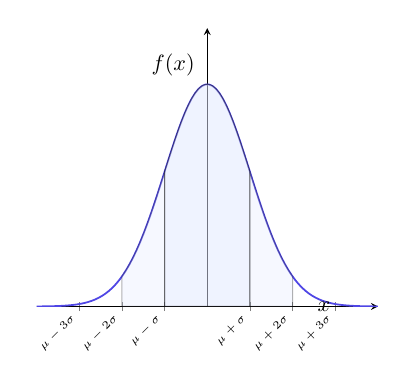
\begin{tikzpicture}[scale=0.8]
\begin{axis}[
    domain=-4:4,
    samples=100,
    axis lines=center,
    xlabel={$x$},
    ylabel={$f(x)$},
    every axis x label/.style={at={(current axis.right of origin)},anchor=west},
    every axis y label/.style={at={(current axis.above origin)},anchor=south},
    height=6cm,
    width=7cm,
    ymax=0.5,
    xtick={-3,-2,-1,0,1,2,3},
    xticklabels={$\mu-3\sigma$,$\mu-2\sigma$,$\mu-\sigma$,$\mu$,$\mu+\sigma$,$\mu+2\sigma$,$\mu+3\sigma$},
    x tick label style={font=\tiny, rotate=45, anchor=east},
    ytick=\empty
]
\addplot[thick, customblue] {1/sqrt(2*pi)*exp(-x^2/2)};

% Shaded areas
\addplot[fill=customlightblue, opacity=0.5, domain=-1:1] {1/sqrt(2*pi)*exp(-x^2/2)} \closedcycle;
\addplot[fill=customlightblue, opacity=0.3, domain=-2:-1] {1/sqrt(2*pi)*exp(-x^2/2)} \closedcycle;
\addplot[fill=customlightblue, opacity=0.3, domain=1:2] {1/sqrt(2*pi)*exp(-x^2/2)} \closedcycle;
\end{axis}
\end{tikzpicture}

\vspace{0.2cm}
\small Bell-shaped, symmetric
\end{center}
\end{column}
\end{columns}
\end{frame}

% Slide 12: The Empirical Rule
\begin{frame}{The Empirical Rule (68-95-99.7 Rule)}

\textbf{For normal distributions:}

\vspace{0.3cm}

\begin{itemize}
\item \textbf{68\%} of data within $\mu \pm 1\sigma$
\item \textbf{95\%} of data within $\mu \pm 2\sigma$
\item \textbf{99.7\%} of data within $\mu \pm 3\sigma$
\end{itemize}

\vspace{0.4cm}

\begin{exampleblock}{Example: Human Height}
Adult male height: $\mu = 175$cm, $\sigma = 7$cm

\vspace{0.3cm}
\begin{itemize}
\item 68\% between 168-182 cm ($\mu \pm 1\sigma$)
\item 95\% between 161-189 cm ($\mu \pm 2\sigma$)
\item 99.7\% between 154-196 cm ($\mu \pm 3\sigma$)
\end{itemize}

\vspace{0.3cm}
\textbf{Implication:} Someone 196cm+ tall is very unusual (top 0.15\%)!
\end{exampleblock}

\vspace{0.3cm}

\begin{alertblock}{}
This is why we consider $|z| > 3$ as potential outliers
\end{alertblock}
\end{frame}

% Slide 13: Standard Normal Distribution
\begin{frame}{The Standard Normal Distribution}

\begin{block}{Definition}
Normal distribution with $\mu = 0$ and $\sigma = 1$: \\
$Z \sim N(0, 1)$
\end{block}

\vspace{0.3cm}

\textbf{Standardization (Z-transformation):}
$$Z = \frac{X - \mu}{\sigma}$$

Any normal distribution can be converted to standard normal!

\vspace{0.3cm}

\textbf{Why this matters:}
\begin{itemize}
\item Tables and software typically give probabilities for $N(0,1)$
\item Allows comparison across different scales
\item Foundation for hypothesis testing (z-tests, t-tests)
\end{itemize}

\vspace{0.3cm}

\begin{exampleblock}{Example}
Height $X \sim N(175, 7^2)$, find $P(X > 185)$: \\
$Z = \frac{185-175}{7} = 1.43$ \\
$P(X > 185) = P(Z > 1.43) = 0.076$ (7.6\%)
\end{exampleblock}
\end{frame}

% Slide 14: Why Normal is Special
\begin{frame}{Why the Normal Distribution is Special}

\textbf{The normal distribution is central to statistics because:}

\vspace{0.3cm}

\begin{enumerate}
\item \textbf{Appears naturally} in many biological phenomena \\
\small Heights, weights, measurement errors

\vspace{0.2cm}
\item \textbf{Mathematical properties} \\
\small Sums of normals are normal, linear combinations of normals are normal

\vspace{0.2cm}
\item \textbf{Central Limit Theorem} \\
\small Averages of \emph{any} distribution approach normal (we'll see this soon!)

\vspace{0.2cm}
\item \textbf{Basis for many tests} \\
\small t-tests, ANOVA, regression all assume normality (of residuals)

\vspace{0.2cm}
\item \textbf{Well-studied} \\
\small Extensive theory, tables, computational tools
\end{enumerate}

\vspace{0.3cm}

\begin{alertblock}{}
\centering
Understanding the normal distribution is \alert{essential} for statistical inference!
\end{alertblock}
\end{frame}


% Slide 16b: CLT - Alternative Formulation
\begin{frame}{Central Limit Theorem: Sum Formulation}
\framesubtitle{CLT for sums of independent random variables}

\begin{block}{Alternative Statement}
Let $X_1, X_2, \ldots, X_n$ be \textbf{independent and identically distributed (i.i.d.)} random variables with mean $\mu$ and variance $\sigma^2$.

\vspace{0.2cm}
Define the sum: $S_n = X_1 + X_2 + \cdots + X_n$

\vspace{0.2cm}
Then as $n \to \infty$:
$\frac{S_n - n\mu}{\sigma\sqrt{n}} \xrightarrow{d} N(0, 1)$

Or equivalently: $S_n \sim N(n\mu, n\sigma^2)$ approximately
\end{block}

\vspace{0.3cm}

\begin{alertblock}{Connection to Sample Mean}
Since $\bar{X} = \frac{S_n}{n}$, dividing by $n$ gives:
$\frac{\bar{X} - \mu}{\sigma/\sqrt{n}} = \frac{S_n - n\mu}{\sigma\sqrt{n}} \sim N(0, 1)$
\end{alertblock}
\end{frame}

% Slide 16c: CLT Intuition
\begin{frame}{Why Does CLT Work? Intuition}

\textbf{Key insight:} When you add many independent random variables, extreme values cancel out

\vspace{0.3cm}

\begin{columns}[T]
\begin{column}{0.48\textwidth}
\textbf{Individual variables:}
\begin{itemize}
\item Can be any distribution
\item High variability
\item Skewed, multimodal, etc.
\end{itemize}

\vspace{0.3cm}
\textbf{Example:}
Single die roll: \\
Uniform on \{1,2,3,4,5,6\}
\end{column}

\begin{column}{0.48\textwidth}
\textbf{Sum/Average:}
\begin{itemize}
\item Becomes bell-shaped
\item Lower relative variability
\item Approaches normal
\end{itemize}

\vspace{0.3cm}
\textbf{Example:}
Sum of 30 die rolls: \\
Approximately $N(105, 87.5)$
\end{column}
\end{columns}

\vspace{0.4cm}

\begin{exampleblock}{Biological Example}
Total biomass of $n$ organisms: each with random mass $X_i$
\begin{itemize}
\item Individual masses: could be any distribution (skewed, etc.)
\item Total biomass $S_n = X_1 + \cdots + X_n$: approximately normal for large $n$
\item Average mass $\bar{X} = S_n/n$: also approximately normal
\end{itemize}
\end{exampleblock}
\end{frame}


% Slide 15: Sampling Distributions
\begin{frame}{From Populations to Samples: Sampling Distributions}

\begin{block}{The Setup}
\begin{itemize}
\item \textbf{Population:} All possible individuals (usually huge/infinite)
\item \textbf{Sample:} Subset we actually observe (limited size $n$)
\item \textbf{Statistic:} Summary of sample (e.g., $\bar{x}$, $s^2$)
\end{itemize}
\end{block}

\vspace{0.3cm}

\begin{block}{Sampling Distribution}
If we took \alert{many different samples} from the same population, \\
the distribution of a statistic (e.g., $\bar{x}$) across those samples
\end{block}

\vspace{0.3cm}

\begin{exampleblock}{Example: Mean Height}
\begin{itemize}
\item Population: All adult males in a country
\item Take 100 different samples, each of size $n = 50$
\item Calculate $\bar{x}$ for each sample
\item Distribution of those 100 means = \alert{sampling distribution of $\bar{x}$}
\end{itemize}
\end{exampleblock}

\vspace{0.2cm}

\textbf{Key insight:} Even if population isn't normal, sampling distribution often is!
\end{frame}

% Slide 16: Central Limit Theorem
\begin{frame}{The Central Limit Theorem (CLT)}
\framesubtitle{The most important theorem in statistics}

\begin{alertblock}{Central Limit Theorem}
For a random sample of size $n$ from \alert{any} distribution with mean $\mu$ and variance $\sigma^2$:

As $n$ increases, the sampling distribution of $\bar{x}$ approaches:
$$\bar{X} \sim N\left(\mu, \frac{\sigma^2}{n}\right)$$

or equivalently:
$$\frac{\bar{X} - \mu}{\sigma/\sqrt{n}} \sim N(0, 1)$$
\end{alertblock}

\vspace{0.3cm}

\textbf{What this means:}
\begin{itemize}
\item Sample mean $\bar{x}$ is approximately normal, \alert{even if population isn't!}
\item Centered at population mean $\mu$
\item Variability decreases as $n$ increases: $\text{SD}(\bar{x}) = \sigma/\sqrt{n}$
\item Usually works well for $n \geq 30$ (sometimes smaller)
\end{itemize}
\end{frame}


% Slide 17: CLT Visualization
\begin{frame}{Central Limit Theorem: Visual Demonstration}

\textbf{Example: Uniform distribution (decidedly not normal!)}

\vspace{0.3cm}

\begin{columns}[T]
\begin{column}{0.48\textwidth}
\textbf{Population (Uniform):}
\begin{center}
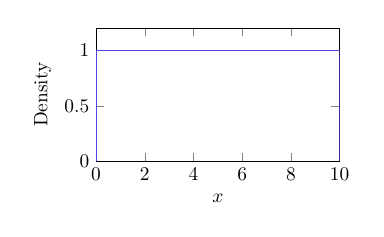
\begin{tikzpicture}[scale=0.7]
\begin{axis}[
    ymin=0, ymax=1.2,
    xmin=0, xmax=10,
    xlabel={$x$},
    ylabel={Density},
    height=4cm,
    width=6cm
]
\addplot[thick, customblue, const plot] coordinates {(0,0) (0,1) (10,1) (10,0)};
\end{axis}
\end{tikzpicture}
\end{center}
Flat, symmetric
\end{column}

\begin{column}{0.48\textwidth}
\textbf{Sampling dist. of $\bar{x}$ ($n=30$):}
\begin{center}
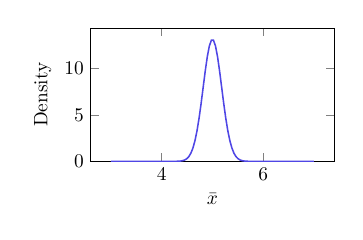
\begin{tikzpicture}[scale=0.7]
\begin{axis}[
    domain=3:7,
    samples=100,
    ymin=0,
    xlabel={$\bar{x}$},
    ylabel={Density},
    height=4cm,
    width=6cm
]
\addplot[thick, customblue] {6*sqrt(30/(2*pi))*exp(-30*(x-5)^2/2)};
\end{axis}
\end{tikzpicture}
\end{center}
Bell-shaped (normal!)
\end{column}
\end{columns}

\vspace{0.4cm}

\begin{block}{The Magic}
Averaging creates normality—\alert{this is why inference works!}
\end{block}
\end{frame}

% Slide 18: Standard Error
\begin{frame}{Standard Error of the Mean}

\begin{block}{Standard Error (SE)}
The standard deviation of the sampling distribution:
$$SE = \frac{\sigma}{\sqrt{n}}$$

If population SD unknown (usual case), estimate with sample SD:
$$SE = \frac{s}{\sqrt{n}}$$
\end{block}

\vspace{0.2cm}

\textbf{Interpretation:}
\begin{itemize}
\item Quantifies uncertainty in our estimate of $\mu$
\item Larger samples → smaller SE → more precise estimate
\item SE decreases with $\sqrt{n}$, not $n$ (diminishing returns!)
\end{itemize}

\vspace{0.3cm}

\begin{exampleblock}{Example}
Measure blood glucose in 25 patients: $\bar{x} = 95$ mg/dL, $s = 15$ mg/dL

\vspace{0.2cm}
$SE = \frac{15}{\sqrt{25}} = 3$ mg/dL

\vspace{0.2cm}
Our estimate of population mean is $95 \pm 3$ mg/dL (roughly)
\end{exampleblock}
\end{frame}

% Slide 19: Sample Size Effects
\begin{frame}{The Effect of Sample Size}

\begin{block}{Key Relationship}
$$SE = \frac{\sigma}{\sqrt{n}}$$

Standard error decreases as sample size increases
\end{block}

\vspace{0.3cm}

\begin{exampleblock}{Numerical Example}
Population SD = 20

\vspace{0.2cm}
\begin{itemize}
\item $n = 4$: $SE = 20/\sqrt{4} = 10$
\item $n = 16$: $SE = 20/\sqrt{16} = 5$ (4x larger $n$ → 2x smaller SE)
\item $n = 100$: $SE = 20/\sqrt{100} = 2$
\item $n = 400$: $SE = 20/\sqrt{400} = 1$ (100x larger $n$ → 10x smaller SE)
\end{itemize}
\end{exampleblock}

\vspace{0.3cm}

\begin{alertblock}{Practical Implication}
To halve the SE, need to \alert{quadruple} the sample size! \\
This is why power analysis is crucial—large samples needed for precision
\end{alertblock}
\end{frame}

% Slide 20: Connecting to Inference
\begin{frame}{Connecting to Statistical Inference}

\begin{center}
\textbf{We now have all the building blocks for inference!}
\end{center}

\vspace{0.3cm}

\begin{block}{What We Know}
\begin{enumerate}
\item Populations have parameters ($\mu$, $\sigma^2$) we want to learn about
\item We observe samples and calculate statistics ($\bar{x}$, $s^2$)
\item Statistics have \alert{sampling distributions} (how they vary across samples)
\item By CLT, $\bar{x}$ is approximately normal with mean $\mu$ and SE $= \sigma/\sqrt{n}$
\end{enumerate}
\end{block}

\vspace{0.3cm}

\begin{alertblock}{Next Step (Day 3)}
Use sampling distributions to:
\begin{itemize}
\item Construct \textbf{confidence intervals} for parameters
\item Test \textbf{hypotheses} about parameters
\item Quantify \textbf{uncertainty} in our conclusions
\end{itemize}
\end{alertblock}

\vspace{0.2cm}

\begin{center}
\textbf{The CLT is the bridge from probability to inference!}
\end{center}
\end{frame}

% Slide 21: Distribution Summary
\begin{frame}{Summary: Key Probability Distributions}

\begin{center}
\small
\begin{tabular}{|l|l|l|p{4.5cm}|}
\hline
\textbf{Distribution} & \textbf{Type} & \textbf{Parameters} & \textbf{Biology Examples} \\
\hline
Binomial & Discrete & $n$, $p$ & Number of mutant offspring; genotype counts; treatment successes \\
\hline
Poisson & Discrete & $\lambda$ & Mutation counts; rare events; cell counts in microscopy \\
\hline
Normal & Continuous & $\mu$, $\sigma^2$ & Height, weight; measurement error; \alert{sampling distributions} \\
\hline
\end{tabular}
\end{center}

\vspace{0.4cm}

\textbf{When to use which:}
\begin{itemize}
\item \textbf{Binomial:} Fixed trials, binary outcome, count successes
\item \textbf{Poisson:} Count rare events in time/space
\item \textbf{Normal:} Continuous measurements; sums/averages (CLT)
\end{itemize}

\vspace{0.3cm}

\begin{alertblock}{}
\centering
Many other distributions exist (exponential, gamma, beta, etc.)—\\
we'll introduce them as needed
\end{alertblock}
\end{frame}

% Slide 22: Key Takeaways
\begin{frame}{Key Takeaways: Probability}

\begin{enumerate}
\item \textbf{Probability quantifies uncertainty}—essential for handling biological variability

\vspace{0.2cm}
\item \textbf{Random variables} have probability distributions that characterize them completely

\vspace{0.2cm}
\item \textbf{Binomial, Poisson, Normal} are the workhorses for biological data

\vspace{0.2cm}
\item \textbf{Normal distribution} is special—appears everywhere due to CLT

\vspace{0.2cm}
\item \textbf{Sampling distributions} describe how statistics vary across samples

\vspace{0.2cm}
\item \textbf{Central Limit Theorem:} Sample means are approximately normal, regardless of population distribution

\vspace{0.2cm}
\item \textbf{Standard Error} quantifies uncertainty in our estimates: $SE = \sigma/\sqrt{n}$

\vspace{0.4cm}

\begin{center}
\colorbox{customblue}{\textcolor{white}{\parbox{0.9\textwidth}{\centering\textbf{These concepts are the mathematical foundation for all of statistical inference}}}}
\end{center}
\end{enumerate}

\end{frame}

% Slide 23: Looking Ahead
\begin{frame}{Looking Ahead to Day 3}

\textbf{Tomorrow we'll use these tools to:}

\vspace{0.3cm}

\begin{block}{Estimation}
\begin{itemize}
\item Construct confidence intervals
\item Quantify precision of our estimates
\item Understand margin of error
\end{itemize}
\end{block}

\begin{block}{Hypothesis Testing}
\begin{itemize}
\item Test claims about populations
\item Calculate p-values
\item Make decisions with controlled error rates
\end{itemize}
\end{block}

\vspace{0.2cm}

\begin{alertblock}{The Connection}
\textbf{Today:} Learned about sampling distributions \\
\textbf{Tomorrow:} Use sampling distributions to make inferences about populations
\end{alertblock}

\vspace{0.1cm}

\begin{center}
Everything we do from here builds on today's foundation!
\end{center}
\end{frame}


\end{document}
